\section{Introduction}
\label{sec:introduction}

\begin{figure}[t]
\centering
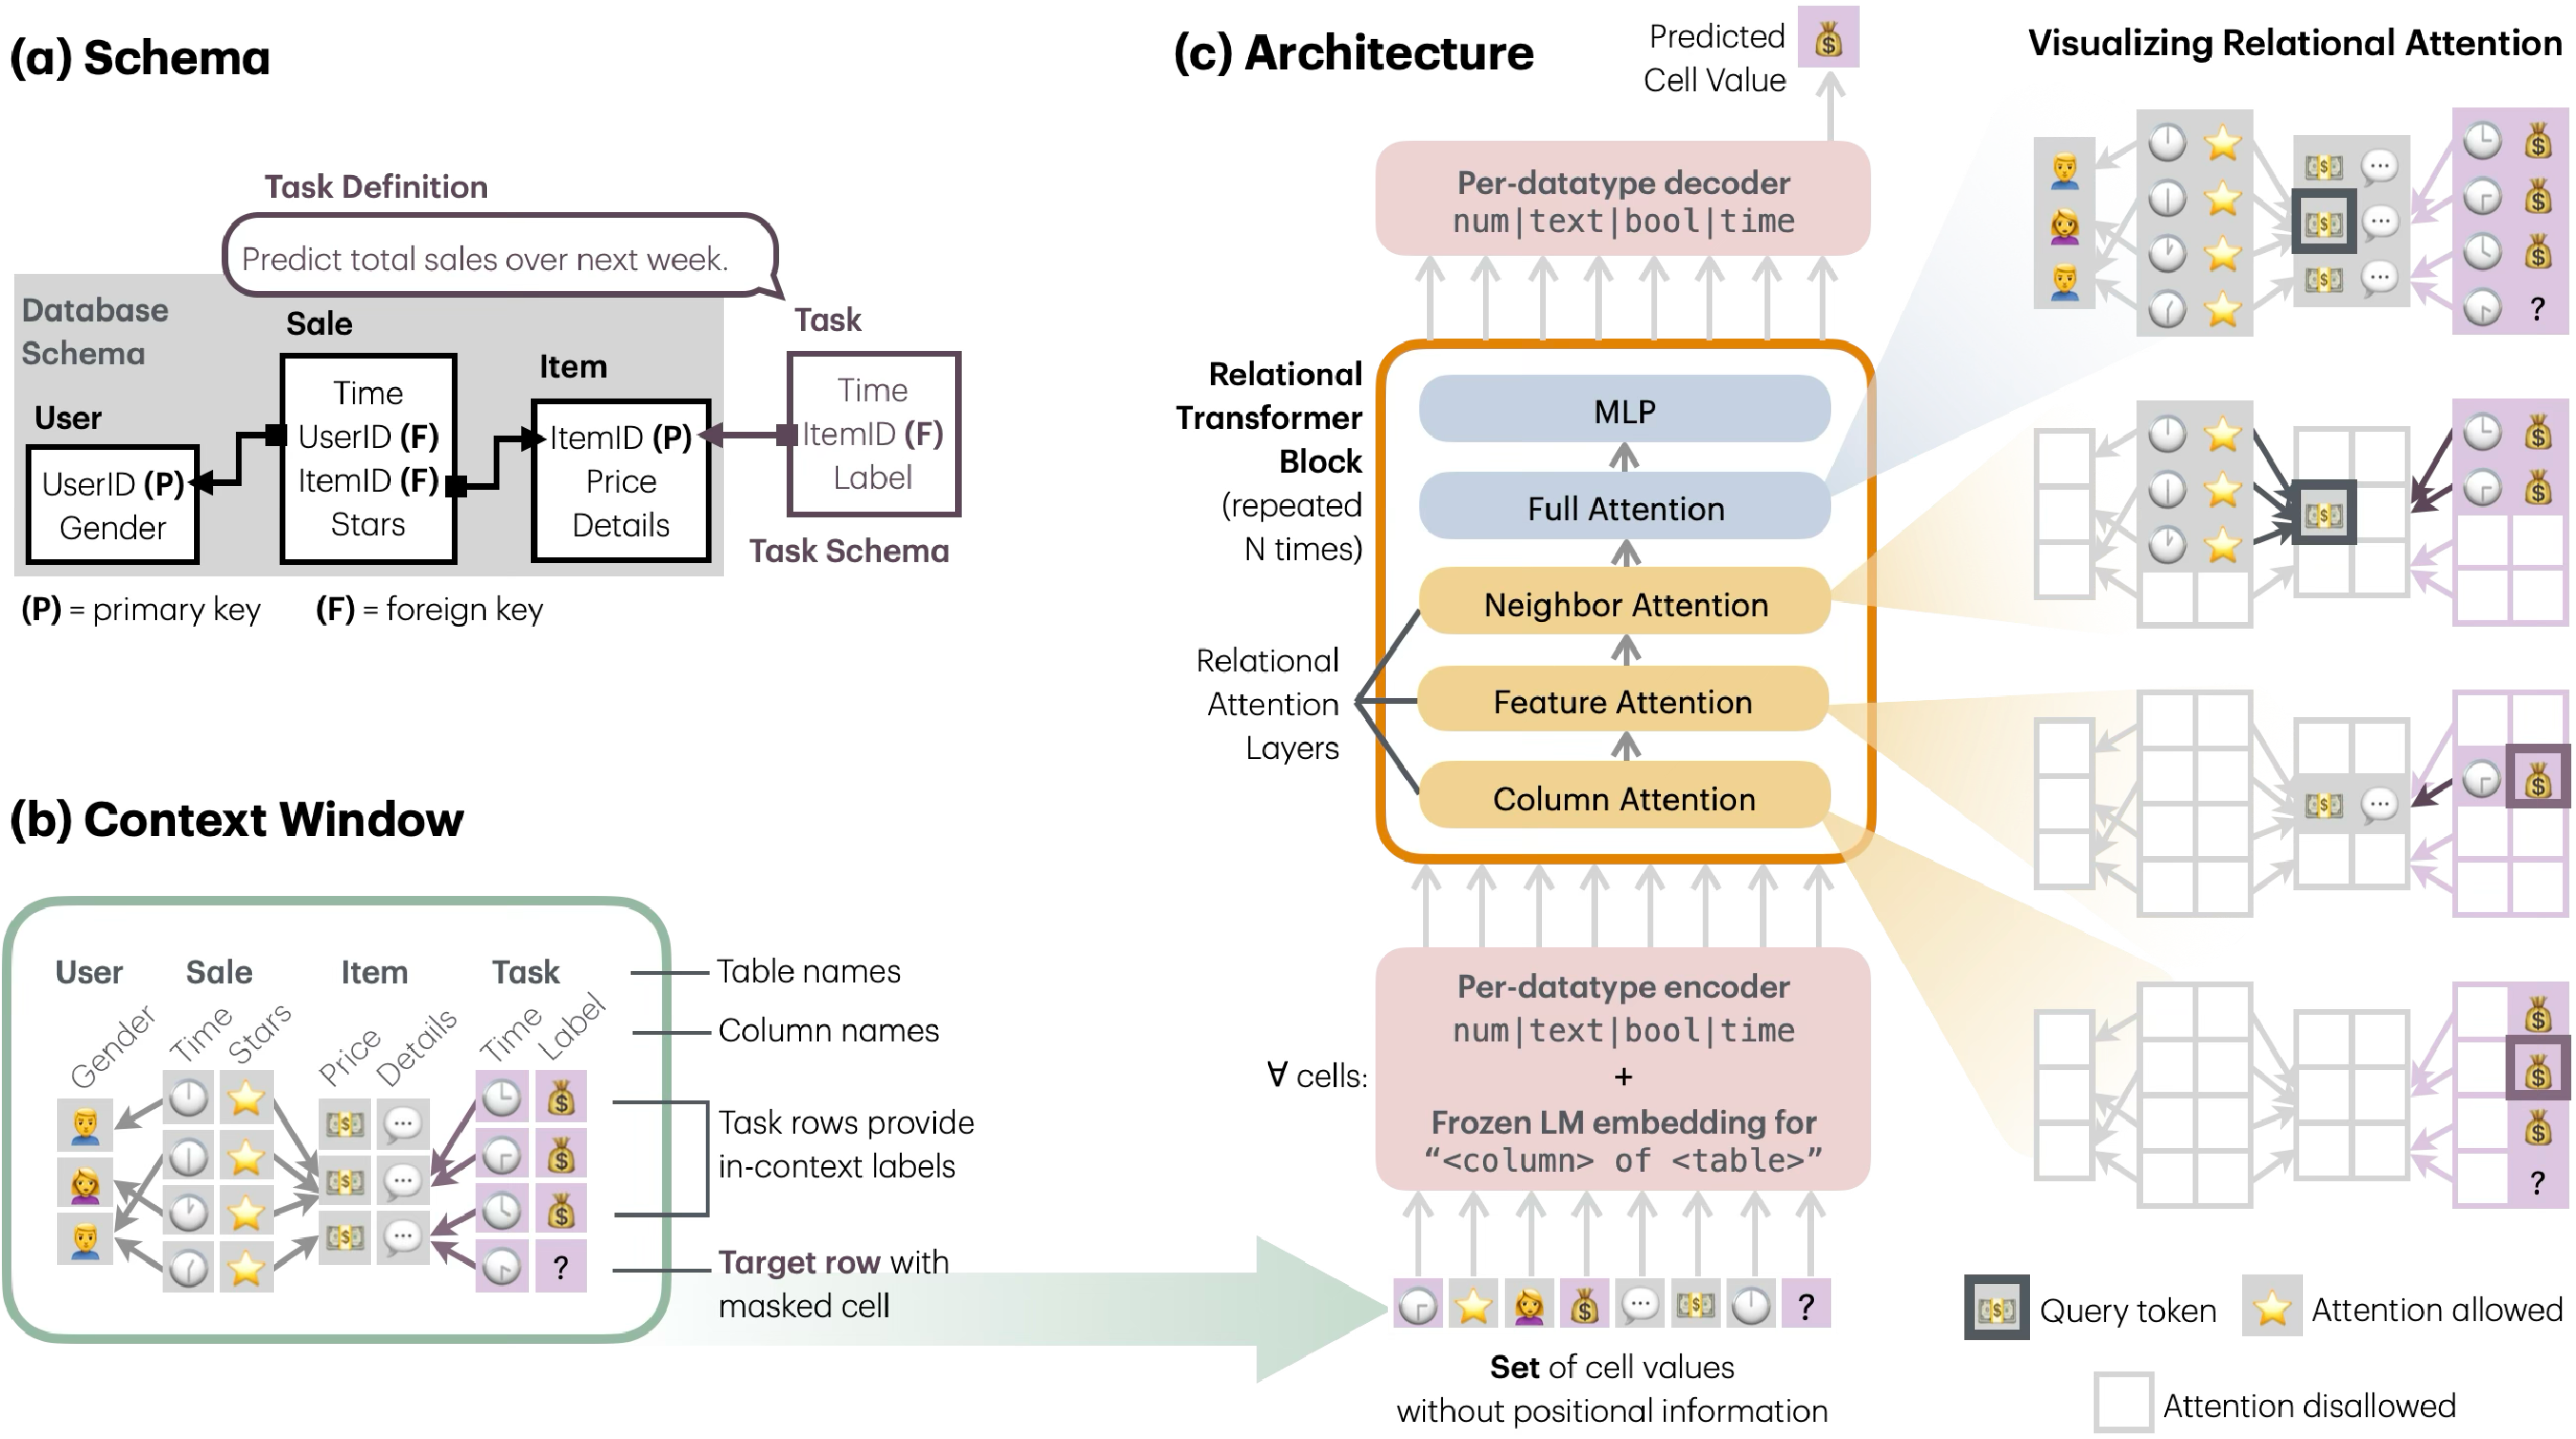
\includegraphics[width=\linewidth]{manual-figures/intro1.pdf}
\caption{
\textbf{(a)}
The \textit{schema} specifies tables, columns,
foreign keys and primary keys.
% A \textit{primary key (P--key)} column uniquely identifies rows in its table.
% A \textit{foreign key (F--key)} column links rows in its table
% to rows in a \textit{parent table},
% by specifying P--key values of parent table rows.
The \textit{task definition} is used to construct the \textit{task table}, which includes labels one aims to predict (e.g., customer churn labels).
\textbf{(b)} The context window captures relevant information to predict the \textit{label column} of the \textit{target row}, which is masked, excluding rows with later timestamps to prevent \textit{temporal leakage}.
See Fig.~\ref{fig:sampler-viz} for a real example.
\textbf{(c)}
Cells correspond to tokens.
Token embedding comprises trainable datatype-specific encoding of cell values
and frozen language model (LM) embeddings of table/column names.
% No positional encodings are used.
Relational structure is modeled by our novel \textit{Relational Attention layers}, where a cell attends to (1) cells in the same column (\textit{column attention}), (2) cells in the same row and F$\to$P linked rows (\textit{feature attention}), and (3) P$\to$F linked rows (\textit{neighbor attention}).
}
\label{fig:intro1}
\end{figure}

% What is the problem?
Foundation models \citep{bommasani2022foundation, zhou2024comprehensive} have redefined natural language processing (NLP)~\citep{bert} and computer vision (CV)~\citep{vit} by demonstrating the effectiveness of general-purpose architectures across diverse domains and tasks. This success is driven by the transformer architecture~\citep{attention}, whose design makes large-scale pretraining possible and yields models that are powerful and broadly transferable. An analogous breakthrough has not yet been achieved for relational data, despite relational databases being the dominant repository of structured enterprise information. Unlike sequences or images, relational databases comprise multiple interconnected tables with heterogeneous columns linked through primary–foreign key relationships. As a result, predictive signal is often scattered across rows, columns, linked tables, and time, making model design substantially more challenging.

% Why is it interesting and important?
% \mf{need to define what you mean by zero-shot manner because neither ICL or fine-tuning are zero-shot.}
Despite its difficulty, designing a foundation model for relational databases is of utmost importance~\citep{vogel2022towards}. Such a model could adapt to new tasks and datasets via zero-shot prompting, few-shot learning or fine-tuning, enabling accurate predictions in cold-start and expertise-, compute- or data-constrained settings. More broadly, it would democratize the use of AI in enterprise contexts, where relational data is ubiquitous, by providing non-experts with accessible predictive tools and offering experts a strong initialization for further model development.

% Why is it hard? (E.g., why do naive approaches fail?)

% See App.~\ref{appsec:related_work} for an expanded discussion.


\paragraph{Prior work.} Traditionally, tasks on relational databases have been solved using tabular models \citep{chen2016xgboost,shwartz2022tabular}, which depend on manual, error-prone, and costly feature engineering~\citep{lam2021automated}. The emerging area of relational deep learning (RDL)~\citep{rdl} addresses this challenge by developing end-to-end models that operate directly on relational databases. Prior RDL research has explored graph neural networks (GNNs)~\citep{relbench,relgnn}, transformers~\citep{relgt, dbformer}, and hybrid models~\citep{relllm} that combine GNNs and large language models (LLMs), to leverage the relational structure. However, these architectures remain tightly coupled to specific schemas and fail to generalize to new databases. In contrast, existing tabular foundation models (TFMs)~\citep{tabpfn, tabpfnv2, carte, tabicl, portal, G2T-FM} generalize to unseen datasets but cannot capture the rich relational structure. 
An alternative is to serialize relational databases into text formats such as XML, JSON, or CSV for processing with LLMs~\citep{snowflake2024relational}, or to flatten them into a single joined table. However, these strategies suffer from scalability issues and distributional mismatch with the pretraining data of LLMs and TFMs. As a result, no existing method provides a viable backbone for building foundation models on relational databases.

% Why hasn't it been solved before?
% (Or, what's wrong with previous proposed solutions? How does mine differ?)


% What are the key components of my approach and results?
% Also include any specific limitations.
\paragraph{Our contribution.} In this paper, we introduce the Relational Transformer (RT) (cf. Fig. \ref{fig:intro1}), a novel transformer design for relational databases that enables large-scale pretraining and zero-shot generalization across diverse domains and tasks. RT introduces three key innovations. First, it represents each database cell as a token, with embeddings constructed from its value, column name and table name.
This cell-level tokenization allows all downstream tasks to be cast as masked token prediction, thereby supporting flexible and scalable self-supervised learning. Second, RT augments the input with task-specific context via \textit{task table prompting}, which enables zero-shot prediction across diverse schemas.
While task rows provide ``in-context labels'',
our setting is not few-shot
as explicit subgraph-label pairs are not required.
Finally, in RT we develop our novel \textit{Relational Attention} mechanism --- \textit{column attention} to model value distributions within a column, \textit{feature attention} to mix information across cells in the same row and their linked parents, and \textit{neighbor attention} to propagate signals along primary–foreign key relationships --- along with the standard self-attention for unrestricted pairwise interactions. Together, these mechanisms capture dependencies across cells, rows, and tables, explicitly leveraging the structure of relational databases.

We pretrain RT on relational databases from RelBench~\citep{relbench}
and observe strong zero-shot transfer to new tasks on unseen datasets.
For example,
average zero-shot AUROC on binary classification tasks
is $90.3\%$ of full supervised learning AUROC,
and rises to $93.1\%$ with continued pretraining on the target dataset
(but not the task).
For comparison,
Gemma3-27B achieves only $83.7\%$ of full supervised learning AUROC
with equivalent context information expressed as text,
despite taking $10^5\times$ more inference FLOPs.
% On regression tasks,
% RT is the only model which achieves better results than
% trivial non-neural baselines in a zero-shot setting.
Further, pretrained RT shows high learning efficiency,
reaching similar performance as the second-best baseline
in $10$--$100\times$ fewer steps / training examples.
These findings establish RT as a powerful model capable of robust zero-shot transfer in relational settings, while enabling rapid fine-tuning when supervision is available. Our results provide strong empirical evidence that relational databases, despite spanning diverse applications, share transferable patterns that can be captured through pretraining.
Overall, this work marks a significant step toward building foundation models for predictive tasks on relational data, moving beyond hand-crafted features and task-specific models to a unified approach for relational modeling.

% \rr{@CK The main contributions of this paper are:}

\begin{figure}[t]
\centering
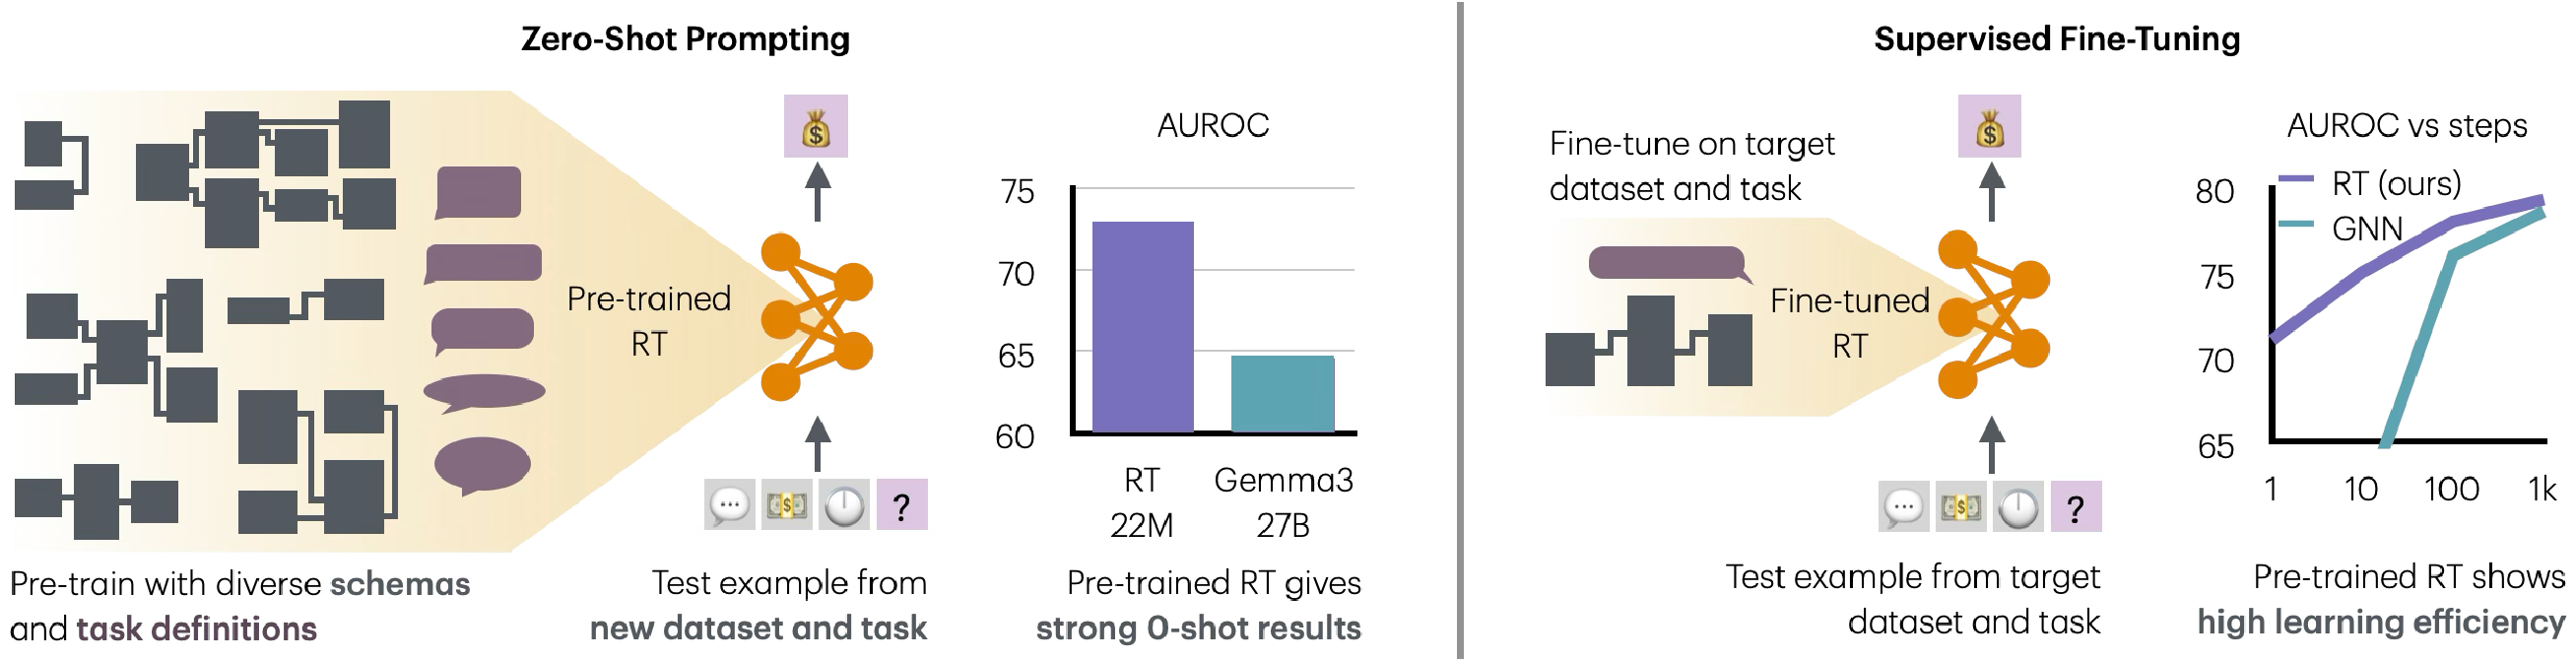
\includegraphics[width=\linewidth]{manual-figures/intro2.pdf}
\caption{
RT can be pretrained on data with diverse schemas and task definitions.
Pretrained RT is accurate on new datasets and tasks with zero-shot prompting.
See Fig.~\ref{fig:sampler-viz} for an example zero-shot prompt.
Dataset- and task-specific fine-tuning of pretrained RT shows
high learning efficiency.
}
\label{fig:intro2}
\end{figure}

